\section{Network Models}
Based on how communication between two machines in a network is achieved, the mode of communication can be classified as connection oriented and connection-less. In connection oriented mode, two machines must establish an implicit connection between them to communicate where as in connection-less mode, communication progresses without establishing implicit connections.

\subsection{Client-Server Model}
The client/server model is a computing model in which clients request services provided by server. A client does not share any of its resources, but requests a server's content or service function. Clients therefore initiate communication sessions with servers which await incoming requests.
\begin{figure}[htbp]
			\begin{center}
			\setlength{\unitlength}{1cm}
			\begin{picture}(12,5)(0,0)
			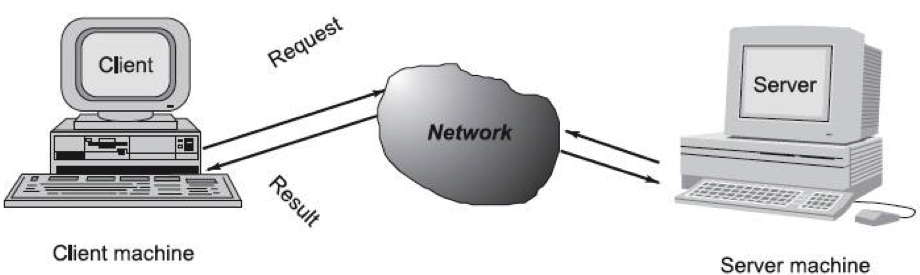
\includegraphics[width=12cm]{./Networking/networking/clientServer.png}
			\end{picture}
	\caption{Client-Server Model}
	\label{ClientServer}
	\end{center}
	\end{figure}
\subsection{Peer-To-Peer Model}
A peer-to-peer (abbreviated to P2P) computer network is one in which each computer in the network can act as a client or server for the other computers in the network, allowing shared access to various resources such as files, peripherals, and sensors without the need for a central server.
P2P is a distributed application architecture that partitions tasks or workloads among peers. Peers are equally privileged participants in the application. Each computer in the network is referred to as a node. The owner of each computer on a P2P network would set aside a portion of its resources - such as processing power, disk storage, or network bandwidth - to be made directly available to other network participant, without the need for central coordination by servers or stable hosts.